% $Header: /u/gcmpack/manual/s_examples/global_oce_optim/global_oce_estimation.tex,v 1.10 2008/01/26 00:27:33 dfer Exp $
% $Name:  $

\section[Global Ocean State Estimation Example]{Global Ocean State Estimation at $4^\circ$ Resolution}
\label{www:tutorials}
\label{sect:eg-global_state_estimate}
\begin{rawhtml}
<!-- CMIREDIR:eg-global_state_estimate: -->
\end{rawhtml}
\begin{center}
(in directory: {\it verification/tutorial\_global\_oce\_optim/})
\end{center}

\subsection{Overview}

Mean surface heat flux as a  control variable : $Q_\mathrm{netm}$

This experiment illustrates the optimization capacity of the MITgcm.
Using an ocean configuration with realistic geography and bathymetry on a
$4\times4^\circ$ spherical polar grid, we estimate a time-independent surface
heat flux adjustment $Q_\mathrm{netm}$ that attempts to bring the model
climatology into consistency with observations (Levitus climatology).
The files for this experiment can be found in the verification directory under
tutorial\_global\_oce\_optim.

This adjustment $Q_\mathrm{netm}$ (a 2D field only function of longitude and
latitude) is the control variable of an optimization problem. It is inferred
by an iterative procedure using an `adjoint technique' and a least-squares
method (see, for example, Stammer et al. (2002) and Ferreira et al. (2005)).

The ocean model is run forward in time and the quality of the solution is
determined by a cost function, $J_1$, a measure of the departure of the model
climatology from observations:
\begin{equation}
J_1=\frac{1}{N}\sum_{i=1}^N \left[ \frac{\overline{T}_i-\overline{T}_i^{lev}}{\sigma_i^T}\right]^2
\end{equation}
where $\overline{T}_i$ is the average model potential temperature and
$\overline{T}_i^{lev}$ the annual mean observed potential temperature at each
grid point $i$. The differences are weighted by an {\it a priori} uncertainty
$\sigma_i^T$ on observations (as provided by Levitus and Boyer 1994). The error
$\sigma_i^T$ is only a function of depth and varies from 0.5 at the surface to
0.05~K at the bottom of the ocean, mainly reflecting the decreasing
temperature variance with depth (Fig. \ref{Error}a). A value of $J_1$ of
order 1 means that the model is, on average, within observational
uncertainties.

The cost function also places constraints on the adjustment to insure it is
"reasonable", i.e. of order of the uncertainties on the observed surface heat
flux: 
\begin{equation}
J_2 = \frac{1}{N} \sum_{i=1}^N \left[\frac{Q_\mathrm{netm}}{\sigma^Q_i} \right]^2
\end{equation}
where $\sigma^Q_i$ are the {\it a priori} errors on the observed heat flux as
estimated by Stammer et al. (2002) from 30\% of local root-mean-square
variability of the NCEP forcing field (Fig \ref{Error}b ).

The total cost function is defined as $J=\lambda_1 J_1+ \lambda_2 J_2$ where
$\lambda_1$ and $\lambda_2$ are weights controlling the relative contribution
of the two components. The adjoint model then yields the sensitivities
$\partial J/\partial Q_\mathrm{netm}$ of $J$ relative to the 2D fields
$Q_\mathrm{netm}$. Using a line-searching algorithm (Gilbert and
Lemar\'{e}chal, 1989), $Q_\mathrm{netm}$ is adjusted then in the sense to
reduce $J$ --- the procedure is repeated until convergence.

In the following example, the configuration is identical to the ``Global Ocean
circulation'' tutorial where more details can be found. In each iteration, the
model is started from rest with temperature and salinity initial conditions
taken from Levitus dataset and run for a year. The first guess
$Q_\mathrm{netm}$ is chosen to be zero. The experiment is run for a year
and the temperature cost function $J_1$ is computed using the annual averaged
potential temperature.

The experiment employs two executables: one for the MITgcm and its adjoint and
one for the line-search algorithm (offline optimization). The implementation
of the control variable $Q_\mathrm{netm}$, the cost function $J$ and the I/O
required for the communication between the model and the line-search are
described in detail in section 2. The compilation of the two executables is
given in section 3. The method used to run the experiment is described in
section 4.

\begin{figure} [tpb]
\begin{center}
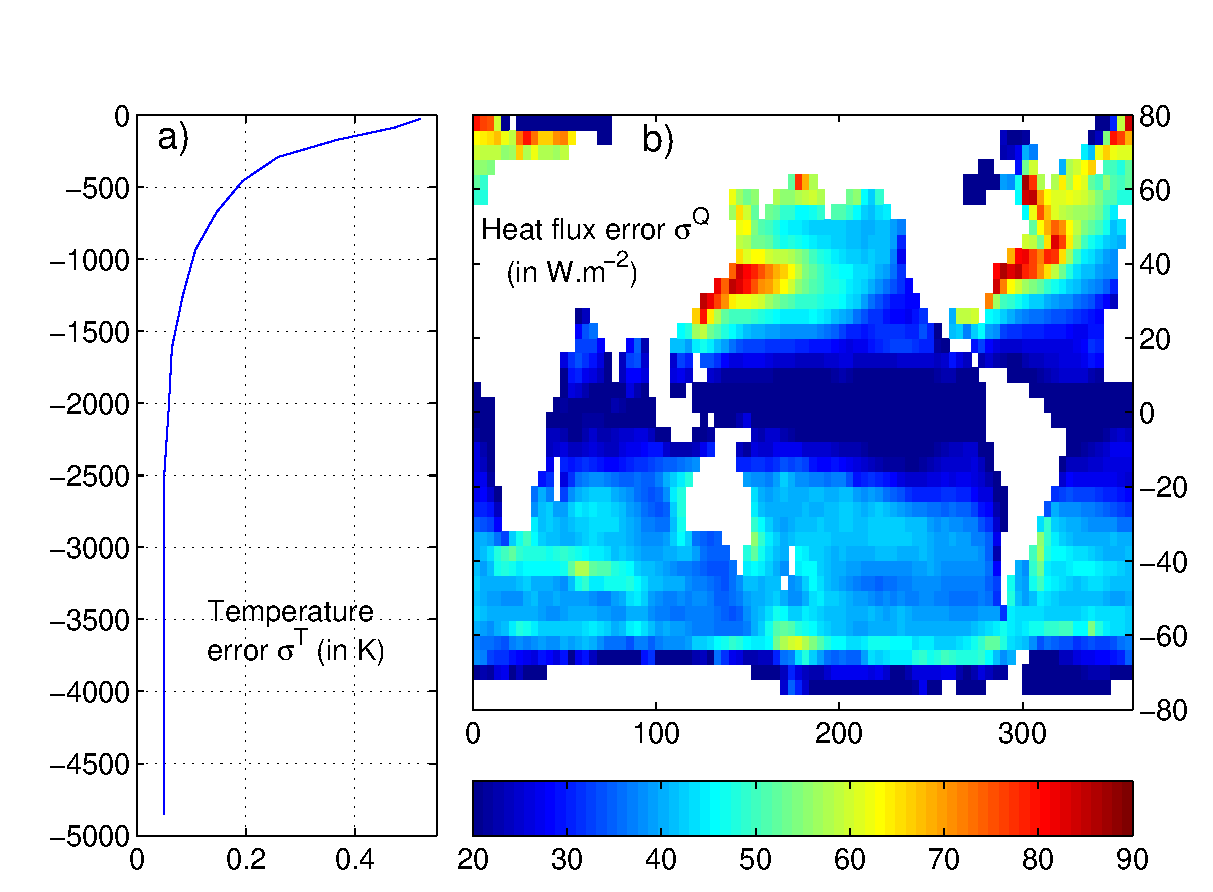
\includegraphics[width=\textwidth,height=.3\textheight]{part3/case_studies/global_oce_estimation/Error.eps}
\caption{{\it A priori} errors used in the cost functions on a) the temperature and b) the surface heat flux.} 
\label{Error}
\end{center}
\end{figure}

Gilbert, J. C., and C. Lemar\'echal, 1989: Some numerical experiments with
variable-storage quasi-Newton algorithms. \textit{Math. Programm.,}
\textbf{45,} 407-435.

\subsection{Implementation of the control variable and the cost function}

All subroutines that require modifications are found in
verifications/Optim/code\_ad

\subsubsection{The control variable}

The adjustment $Q_\mathrm{netm}$ is activated by setting
ALLOW\_HFLUXM\_CONTROL to "define" in ECCO\_OPTIONS.h.

It is first implemented as a ``normal'' forcing variable. It is defined in
FFIELDS.h, initialized to zero in ini\_forcing.F, and then used in
external\_forcing\_surf.F. $Q_\mathrm{netm}$ is made a control variable in
the ctrl package by modifying the following subroutines:

\begin{itemize}
\item ctrl\_init.F where $Q_\mathrm{netm}$ is defined as the control variable
number 24,

\item ctrl\_pack.F which writes, at the end of each iteration, the sensitivity
of the cost function $\partial J/\partial Q_\mathrm{netm}$ in to a file to be
used by the line-search algorithm,

\item ctrl\_unpack.F which reads, at the start of each iteration, the updated
perturbations as provided by the line-search algorithm,

\item ctrl\_map\_forcing.F in which the updated perturbation is added to the
first guess $Q_\mathrm{netm}$.
\end{itemize}

Note also some minor changes in ctrl.h, ctrl\_readparams.F, and ctrl\_dummy.h
(xx\_hfluxm\_file, fname\_hfluxm, xx\_hfluxm\_dummy).

\subsubsection{Cost functions}

The cost functions are implemented using the {\it cost} package.

\begin{itemize}

\item The temperature cost function $J_1$ which measures the drift of the mean
model temperature from the Levitus climatology is implemented cost\_temp.F.
It is activated by ALLOW\_COST\_TEMP in ECCO\_OPTIONS.h. It requires the mean
temperature of the model which is obtained by accumulating the temperature in
cost\_tile.F (called at each time step).
The value of the cost function is stored in {\it objf\_temp} and its weight
$\lambda_1$ in {\it mult\_temp}.

\item The heat flux cost function, penalizing the departure of the surface
heat flux from observations is implemented in cost\_hflux.F, and activated by
activated ALLOW\_COST\_HFLUXM in ECCO\_OPTIONS.h. The value of the cost
function is stored in {\it objf\_hfluxm} and its weight $\lambda_2$ in
{\it mult\_hfluxm}.

\item The subroutine cost\_final.F calls the cost\_functions subroutines
and make the (weighted) sum of the various contributions.

\item The various weights used in the cost functions are read in
cost\_weights.F. The weight of the cost functions are read in
cost\_readparams.F from the input file data.cost.    

\end{itemize}


\subsection{Code Configuration}
\label{www:tutorials}
\label{SEC:eg_fourl_code_config}

The model configuration for this experiment resides under the directory
{\it verification/tutorial\_global\_oce\_optim/}.  The experiment files in
code\_ad/ and input\_ad/ contain the code customizations and parameter
settings. Most of them are identical to those used in the Global Ocean
experiment. Below we describe the customizations to these files required for
the experiment.

\subsubsection{Compilation-time customizations in {\it code\_ad/}}

ECCO_CPPOPTIONS.h the optimization.

\begin{itemize}
\item ALLOW\_ECCO\_OPTIMIZATION

\item ALLOW\_COST ALLOW\_COST\_TEMP ALLOW\_COST\_HFLUXM

\item ALLOW\_HFLUXM\_CONTROL
\end{itemize}

\subsubsection{Running-time customizations in {\it input\_ad/}}

\begin{itemize}

\item {\it data} is similar to 

\item {\it data.optim} specifies the iteration number.

\item {\it data.ctrl} is used, in particular, to specify the
name of the sensitivity and adjustment files associated to a control
variable.

\item {\it data.cost} 

\item {\it data.pkg}

\item {\it Err\_hflux.bin} and {\it Err\_levitus\_15layer.bin} are the
files containing the heat flux and potential temperature uncertainties,
respectively.

\item {\it Err\_levitus\_15layer.bin}

\item Subdirectory {\it OPTIM}

\end{itemize}

\subsection{Compiling} 

The optimization experiment requires two executables: 1) the 
MITgcm and its adjoint ({\it mitgcmuv\_ad}) and 2) the line-search
algorithm ({\it optim.x}).

\subsubsection{Compilation of MITgcm and its adjoint: {\it mitcgmuv\_ad}}

Before compiling, first note that, in the directory code\_ad/, two files
must be updated:
\begin{itemize}
\item code\_ad\_diff.list which lists new subroutines to be compiled
by the TAF software (cost\_temp.F and cost\_hflux.F here),

\item  the adjoint\_hfluxm files which provides a list of the control variables
and the name of cost function to the TAF software.

\end{itemize}

Then, in the directory build\_ad/, type:
\begin{verbatim}
% ../../../tools/genmake2 -mods=../code\_ad -adof=../code\_ad/adjoint\_hfluxm
% make depend
% make adall
\end{verbatim}
to generate the MITgcm executable {\it mitgcmuv\_ad}.

\subsubsection{Compilation of the line-search algorithm: {\it optim.x}}

This is done from the directories lsopt/ and optim/ (under MITgcm/). In lsopt/,
unzip the blash1 library adapted to your platform, and change the Makefile
accordingly. Compile with:
\begin{verbatim}
% make all
\end{verbatim}
(more details in lsopt\_doc.txt)

In optim/,  the path of the directory where {\it mitgcm\_ad} was compiled
must be specified in the Makefile in the variable INCLUDEDIRS. The file name
of the control variable (xx\_hfluxm\_file here) must be added to the name list
read by optim\_num.F. Then use
\begin{verbatim}
% make depend
\end{verbatim} 
and
\begin{verbatim}
% make
\end{verbatim}
to generate the line-search executable {\it optim.x}.

\subsection{Running the estimation}

Copy the {\it mitgcmuv\_ad} executable to input\_ad/ and {\it optim.x} to the
subdirectory input\_ad/OPTIM/. Move into input\_ad/. The first iteration is
somewhat particular and is best done "by hand" while the following iterations
can be run automatically (see below). Check that the iteration number is set
to 0 in data.optim and run the MITgcm:
\begin{verbatim}
% ./mitgcmuv_ad
\end{verbatim}

The output files adxx\_hfluxm.0000000000.* and xx\_hfluxm.0000000000.* contain
the sensitivity of the cost function to $Q_\mathrm{netm}$ and the perturbations
to $Q_\mathrm{netm}$ (zero at the first iteration), respectively. Two other
files called ecco\_cost.. and ecco\_ctrl are also generated. They essentially
contain the same information as the adxx\_* and xx\_* files, but in a
compressed format. These two files are the only ones involved in the
communication between the adjoint model {\it mitgcmuv\_ad} and the line-search
algorithm {\it optim.x}. The ecco\_cost*n is an output of the adjoint model at
iteration $n$ and an input of the line-search. The latter returns an updated
perturbation in ecco\_ctrl*n+1 to be used as an input of the adjoint model at
iteration n+1. 

At the first iteration, move these two files (ecco\_cost and ecco\_ctrl) to
OPTIM/, open data.optim and check the iteration number is set to 0. The target
cost function {\it fmin} needs to be specified too: a rule of thumb suggests
it should be set to about 0.95-0.90 times the value of the cost function at
the first iteration. This value is only used at the first iteration and does
not need to be updated afterward. However, it implicitly specifies the
``pace'' at which the cost function is going down (if you are lucky and it does
indeed diminish!). More in the ECCO section maybe ?

Once this is done, run the line-search algorithm:
\begin{verbatim}
% ./optim.x
\end{verbatim}
which computes the updated perturbations for iteration 1 ecco\_ctrl\_1.

The following iterations can be executed automatically using the shell
script {\it cycsh} found in input\_ad/. This script will take care of changing
the iteration numbers in the data.optim, launch the adjoint model, clean and
store the outputs, move the ecco\_cost* and ecco\_ctrl* files, and run the
line-search algorithm. Edit {\it cycsh} to specify the prefix of the
directories used to store the outputs and the maximum number of iteration.
